\chapter{Implementace}\label{chapter-implementation}

V úvodu této kapitoly popíšeme koncepci programu, co kde
běží a jakým způsobem spolu komunikuje. Následně v sekci~\ref{analysis}
rozebereme zvolenou platformu a programovací jazyky,
další sekce budou pak věnovány popisu komponent, které jsme museli
naimplementovat pro funkci celého systému. Konkrétně jde o aplikaci pro
mobilní telefony s operačním systémem Android (naše implementace,
v sekci~\ref{app}), vytvoření instance WA pro řízení
dialogu (náš návrh za využití existujícího WA,
s popisem získání nejběžnějších českých jmen pro trénink, \ref{wainit}) a komponenty
pro porovnání entit nalezených pomocí WA se seznamem kontaktů (naše implementace,
\ref{matching}).

Výsledkem je z uživatelského pohledu mobilní
aplikace. Většina vnitřních procesů však probíhá v cloudu, aplikace
je jen jakýmsi spojem a médiem pro komunikaci s uživatelem. Celý běh
je znázorněn na obrázku~\ref{img-flowchart}. Stisknutím tlačítka v
telefonu se
inicializuje session ve WA běžícím v cloudu IBM a spustí rozpoznávání řeči,
které běží na serverech Google. Po zahájení session ve WA jsou tam též
odeslána jména kontaktů uložených v telefonu. Jakmile je z hlasu rozpoznán
text, je vrácen zpět do aplikace a odtud odeslán jako zpráva do WA.
Ten rozhodne, zda je potřeba volat
porovnávací komponentu. Pokud ano, zavolá ji z jiné části IBM cloudu,
předá jí relevantní data a získá od ní odpověď. V každém případě
WA vygeneruje odpověď na zaslanou zprávu a odešle ji zpět do telefonu.
Tam je odpověď z WA zpracována (mj. je rozhodnuto, zda by měl být
zahájen hovor) a odeslána do syntetizátoru řeči na servery Google.
Odtud je hlas k přehrání vrácen zpět do aplikace, tam je přehrán
a následně je na základě dřívějšího rozhodnutí buď spuštěno znovu
rozpoznání hlasu, nebo je zahájen hovor a aplikace ukončena.


\begin{figure}[h]
    \centering
    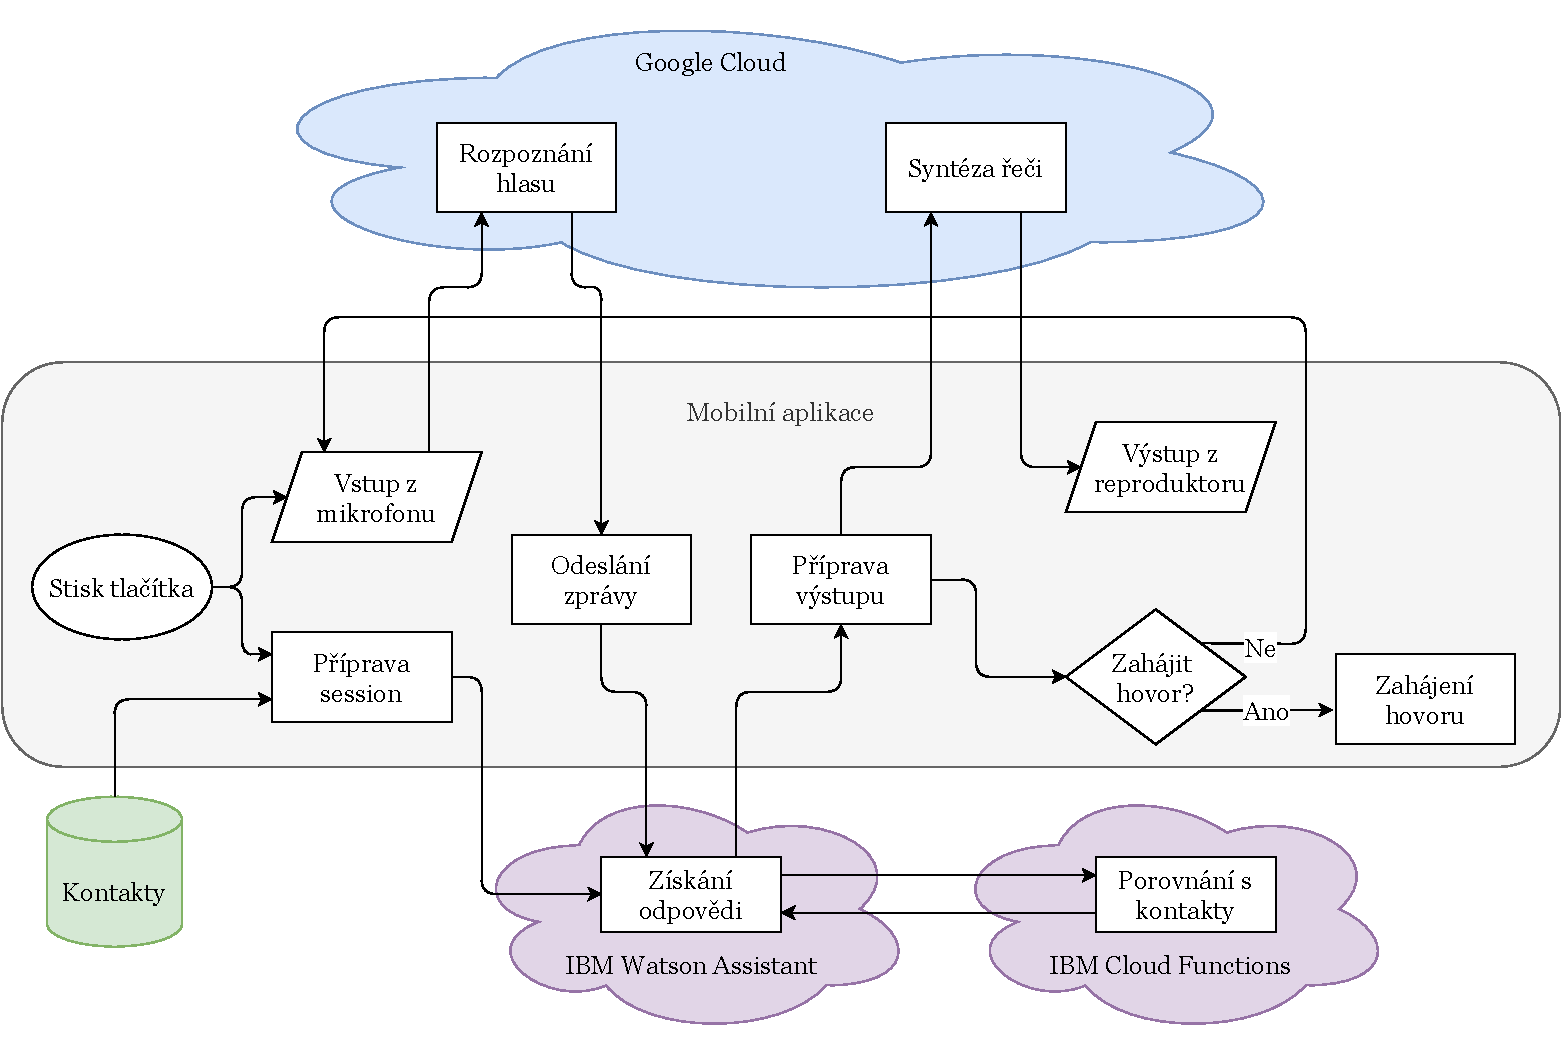
\includegraphics[width=0.98\textwidth]{../img/app-flowchart.pdf}
    \caption{Nákres fungování celého systému.}
    \label{img-flowchart}
\end{figure}

\section{Platforma a programovací jazyky}\label{analysis}

\subsection{Platforma a jazyk mobilní aplikace}
Pro mobilní aplikace máme v dnešní době v zásadě dvě možnosti, iOS nebo Android.
Zvolili jsme Android, neboť je celkově otevřenější, autor telefon s tímto
operačním systémem vlastní a má tedy alespoň uživatelské zkušenosti. IBM navíc
poskytuje vývojový balíček (\textit{SDK}) pro použití WA v programovacím
jazyku Java, který je použitelný i v Androidu.

Z hlediska programovacího jazyka padla volba na Kotlin. Existují různé frameworky
schopné zkompilovat pro Android program psaný téměř v libovolném programovacím
jazyce, ale většina nakonec musí používat nějakou další překladovou vrstvu.
Kotlin je jeden z jazyků, ve kterém lze psát nativní aplikace pro Android. Programy
v něm napsané lze totiž zkompilovat pro spuštění v \textit{JVM} (\textit{Java Virtual Machine}),
toto prostředí popisuje \citet{prof_tejinder_singh_hotspot_2014}.
Kotlin dokonce umožňuje interoperabilitu s Javou, což umožnilo
využití zmíněného SDK. Jeho výhoda oproti Javě je, že je celkově modernější,
psaní a čtení programů v něm je díky přehlednější syntaxi jednodušší a kratší,
navíc je doporučený samotnou firmou Google jakožto vedoucím vývoje operačního
systému Android \citep{android_blog}.
Další vlastností, na kterou při výběru nebyl brán tak velký
zřetel, ale nakonec se ukázala jako relativně zásadní, je podpora \textit{koprogramů}
(\textit{coroutines}), jejichž možnou implementaci ukazují \citet{theory_practice_coroutines}.

\subsection{Volba asistenta a jeho inicializace}
Frameworků pro tvorbu asistentů existuje na trhu mnoho, jen jeden však aktuálně oficiálně plně
podporuje český jazyk -- Watson Assistant od IBM. Proto zde volba jednoduše
padla právě na něj. Představili jsme ho v kapitole~\ref{chapter-wa}.

Nastavení WA lze provést v interaktivním prostředí v prohlížeči. Toto
prostředí je však v mnohém omezené. V našem případě jsme například potřebovali
vložit stovky entit pro trénování rozpoznání. Přenést je do WA přes prohlížeč
by bylo absurdně náročné, navíc složitě replikovatelné. Použili jsme proto opět
po SDK, pomocí kterého můžeme WA nastavit relativně krátkým skriptem. Na volbě
konkrétního programovacího jazyka zde téměř nezáleželo (skript je krátký a běží
jen jednou), zvolili jsme proto Python jakožto dobře čitelný
jazyk, se kterým máme mnoho zkušeností.

\subsection{Jazyk a prostředí běhu porovnávací komponenty}

Volba jazyka byla zde také jednoduchá, neboť má být obecně využitelná v rámci
knihovny \texttt{mConversation} firmy MAMA AI a požadovaným jazykem byl Python.

Pro implementaci jsme potřebovali zjišťovat podobnost řetězců. Algoritmus
zjišťující Levenshteinovu vzdálenost (představili jsme v podsekci~\ref{nlu})
je relativně komplikovaný a běžně používaný, nedávalo tedy
smysl programovat jej znovu. Využili jsme modul
\texttt{editdistance}\footnote{\url{https://pypi.org/project/editdistance/}},
protože je psaný v rychlejším jazyce C++ a má vhodnou licenci.

Dále bylo potřeba vyřešit, kde tato komponenta poběží. Nakonec jsme vybrali
službu IBM Cloud Functions. Původním nápadem bylo
zprovoznění webového serveru, který by vyřizoval požadavky na tuto komponentu.
To by však vyžadovalo další kód pro správu a především hardware, na kterém by
tento server běžel. Při hledání alternativ jsme dostali doporučení na
\textit{funkce poskytované jako služby} (\textit{function as a service, FaaS}),
které nabízí většina větších poskytovatelů cloudů. Jednoduše řečeno, na daný
server lze nahrát kód, který přijímá a vrací (obvykle) soubory formátu JSON a
běží jen ve chvíli, kdy dostane nějaký požadavek. Liší se tak od standardních
webových serverů, které musí \uv{poslouchat} neustále. Konkrétně byla vybrána
služba IBM Cloud Functions především proto, že lze spravovat ze stejného účtu jako
WA. Teoreticky může být výhoda využití stejného poskytovatele ještě v tom, že
servery budou na stejném místě a tedy výměna dat mezi nimi bude probíhat rychleji.

\section{Mobilní aplikace}\label{app}

Pro vytvoření aplikace jsme využili integrované vývojové prostředí
\textit{Android Studio}, které pro kompilaci využívá \textit{gradle}.
Původním záměrem bylo využít \textit{Visual Studio Code}
spolu s \textit{vývojovými kontejnery} za použití virtualizačního softwaru
\textit{Docker}, především díky přenositelnosti a relativní nenáročnosti
na výpočetní výkon. Ukázalo se však, že tato cesta není při vývoji aplikací
pro Android v jazyce Kotlin pod operačním systémem Windows úplně běžná a
naráží na mnoho komplikací. Od ruční inicializace projektu a vytvoření všech
potřebných souborů, přes design uživatelského
prostředí nutný čistě v textovém editoru a složitou správu závislostí,
až po problémy při kompilaci. Nakonec jsme tedy tuto cestu opustili a
musíme konstatovat, že především pro vývojáře začínající s Androidem
ji považujeme za silně nevhodnou.

Aplikace musela vyřešit několik věcí, které popisujeme
v následujících podsekcích: získat oprávnění ke všem operacím (podsekce~\ref{get-permissions}),
získat kontakty uživatele (\ref{get-contacts}), vytvořit \textit{session} ve WA a odeslat
tam jména kontaktů (\ref{create-session}), spustit rozpoznání hlasu (\ref{start-tts}), po dokončení odeslat jeho výsledek
jako zprávu do WA (\ref{contact-wa}), po získání odpovědi spustit hlasový syntetizátor (\ref{start-tts}), po skončení
jeho projevu buď spustit rozpoznání hlasu a celý běh znovu, nebo zahájit
hovor. Všemi součástmi se budeme zabývat v následujících podsekcích, začneme
ale celkovou koncepcí a vzhledem (\ref{desc-ui}).

\subsection{Uživatelské rozhraní}\label{desc-ui}

Protože primárním způsobem interakce
s aplikací má být hlas, cílili jsme na jednoduché a sebevysvětlující grafické
rozhraní. Zvolili jsme tlačítko se symbolem mikrofonu na černém pozadí,
jak ukazuje obrázek~\ref{img-ui}. Tímto tlačítkem je zahájen dialog (v případě
dostatečných oprávnění). Při běhu aplikace
pak obrázkem na něm indikujeme přijímání vstupu (mikrofon se změní na
plný červený) či čtení výstupu (místo mikrofonu se objeví symbol reproduktoru).

\begin{figure}[h]
    \centering
    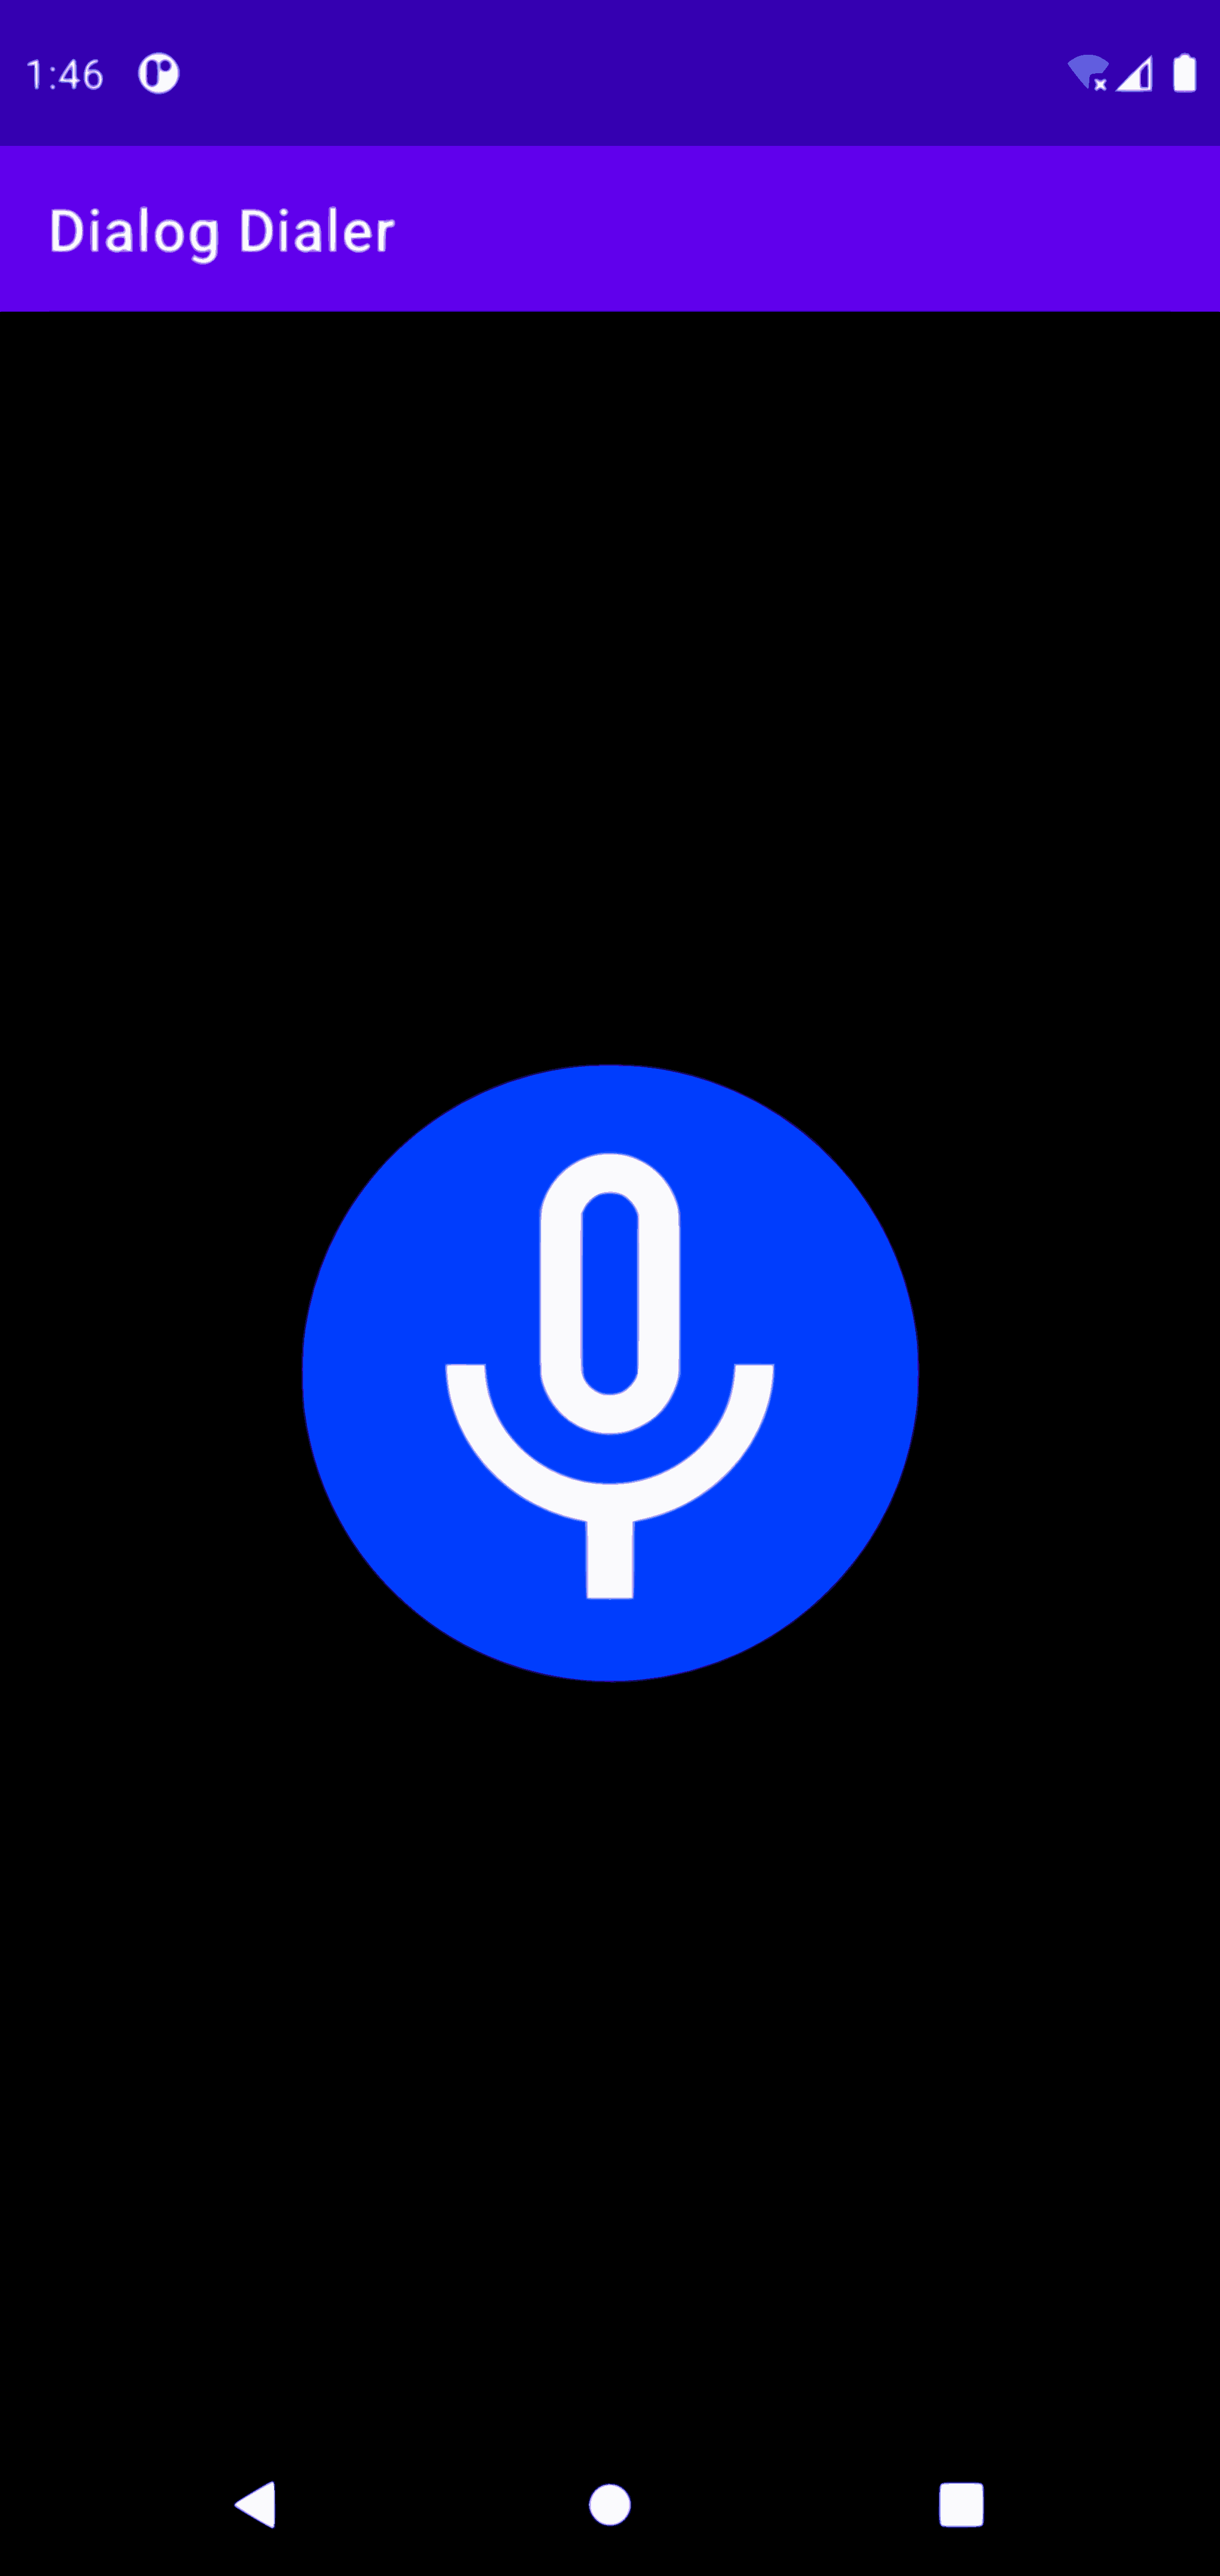
\includegraphics[width=0.3\textwidth]{../img/ui.pdf}
    \caption{Jednoduché uživatelské rozhraní.}
    \label{img-ui}
\end{figure}

\subsection{Získání oprávnění}\label{get-permissions}

Pro svou správnou funkci potřebuje aplikace povolení nahrávat zvuk, číst
kontakty, vykonávat hovory a přistupovat k internetu. První
tři jsou navíc oprávněními za času běhu, tedy o ně musíme explicitně
požádat. Oprávnění k přístupu k internetu nepovažuje Android za tak zásadní (především
protože neoperuje s uživatelovými daty), tedy je automaticky
uděleno při instalaci aplikace.

Aktuálně oficiálně doporučený postup získání oprávnění, kterým se řídíme, popisuje
dokumentace \citet{android_request_permissions}. Nejprve je o ně třeba
požádat, pokud uživatel odmítne a pokusí se
aplikaci znovu použít, zobrazit vysvětlení, k čemu jsou nutná a znovu o ně
požádat, a pokud znovu odmítne, již jen ukazovat upozornění o nedostupnosti.

\subsection{Získání kontaktů}\label{get-contacts}

Kontakty potřebujeme získat z úložiště telefonu, které se chová podobně jako
databáze. Proto dotaz na ně začneme na začátku inicializace celé služby WA
asynchronně jako koprogram. V rámci něj pak získáme jména a čísla kontaktů,
vše uložíme do slovníku.

\subsection{Vytvoření session ve WA a odeslání jmen kontaktů}\label{create-session}

Po začátku dotazu na kontakty vytvoříme instanci třídy \texttt{Assistant}
z Java SDK\footnote{\url{https://github.com/watson-developer-cloud/java-sdk}}
pro komunikaci s WA API, které předáme potřebné parametry a následně pošleme
požadavek pro zahájení session. V Androidu není možné posílat síťové požadavky
v hlavním vlákně (protože je potřeba udržovat ho volné pro UI), takže s výhodou
opět použijeme běh jako koprogram. Následně zajistíme
kontrolu dokončení získávání kontaktů a předáme je jako \textit{kontext} do
WA session. Pokud se v průběhu něco nepovede, výjimku odchytíme a příště
se pokusíme provést celou inicializaci znovu.

Původní záměr byl odesílat kontakty do WA jako standardní zprávu, jenže
tam jsme brzy narazili na limit velikosti požadavku 2048 znaků. Delší
seznam kontaktů se do tohoto limitu nevejde, proto jsme nakonec využili
nastavení kontextu.

\subsection{Spuštění rozpoznávání hlasu}\label{start-tts}

Využijeme vestavěný \texttt{RecognizerIntent.ACTION\_RECOGNIZE\_SPEECH}%
\footnote{\url{https://developer.android.com/reference/android/speech/RecognizerIntent\#ACTION\_RECOGNIZE\_SPEECH}}
nastavený na češtinu. Rozpoznávání hlasu je delší aktivita, takže nemůžeme
aktivně čekat na její
dokončení. Místo toho registrujeme zpětné volání na výsledek aktivity.
Po získání výsledku zkontrolujeme, že proběhla úspěšně a pokud ano, pokračujeme
k dalšímu kroku.

\subsection{Odeslání do WA a získání odpovědi}\label{contact-wa}
Nejdříve ověříme nachystání WA. Pokud je vše připraveno,
pošleme v koprogramu (jedná se o síťový požadavek) text do WA a získáme odpověď.
Protože dialog řídí WA, potřebovali jsme v něm nějakým způsobem aplikaci
předat informaci, že má zahájit hovor a komu má volat. Rozhodli jsme se na první
řádek takové odpovědi umístit řetězec \texttt{[call]}, na druhý řádek jméno kontaktu
a na třetí zprávu pro uživatele. Tak nám v aplikaci stačí kontrolovat první řádek získané
odpovědi a podle něj se rozhodnout. Pomocí jména kontaktu pak zjistíme jeho číslo
a zapamatujeme si, že nemáme znovu spouštět běh pipeline. Podle prvního řádku
pak část nebo celou odpověď pošleme do TTS.

\subsection{Spuštění hlasového syntetizátoru}\label{start-tts}

K převodu textu na řeč použijeme instanci vestavěné
třídy \texttt{TextToSpeech},%
\footnote{\url{https://developer.android.com/reference/android/speech/tts/TextToSpeech}}
kterou vytvoříme při otevření programu. Nastavíme
ji na český jazyk a přepíšeme v ní funkci \texttt{onDone}, která je spuštěna,
když skončí přehrávání hlasu. Pokud dialog neskončil, spustíme celou pipeline
pomocí obalovací funkce \texttt{launchPipeline} znovu. Pokud
skončil, jsme připraveni začít volat, vytočíme tedy číslo a ukončíme session ve
WA i celou aplikaci.

\section{Implementace dialogu ve WA}\label{wainit}

WA v našem programu využíváme pro řízení dialogu. Potřebuje tedy dokázat
rozpoznávat úmysly a entity (rozebíráme v podsekci~\ref{intents-entities}),
v případě nutnosti zavolat porovnávací komponentu, a vybrat na základě
rozpoznaného správnou odpověď (popisujeme v podsekci~\ref{building-dialog}).

\subsection{Úmysly a entity}\label{intents-entities}

Zásadní je úmysl
\texttt{dial}, pomocí kterého detekujeme, že uživatel chce někomu volat. Pro
každý úmysl přidáme několik vzorových vět, na základě kterých by ho měl WA
rozpoznat. Ty jsou interně použity pro trénink modelu stojícího za WA, jak
jsme popsali v sekci~\ref{wa-inside}.
Obdobně vytvoříme zbývající úmysly \texttt{greet} a \texttt{bye}, aby náš
asistent uměl slušně pozdravit.

Jediné entity, které potřebujeme rozeznávat, jsou jména lidí, případně příjmení.
Uvažovali jsme, jak tato
data získat. Nakonec jsme využili data četnosti jmen a příjmení MVČR z roku 2017.
Sice již přímo na stránkách MVČR nejsou dostupná, ale ve ve webových archivech
existují \citep{mvcr_cetnost_2018}. Z nich jsme pomocí krátkého skriptu vybrali
všechna jména i příjmení, která v Česku k roku 2017 nosilo alespoň
200 lidí, a ta jsme nahráli do WA.

\subsection{Stavba dialogu}\label{building-dialog}

Jak jsme popsali v sekci~\ref{wa-create}, je využívána stromová reprezentace dialogu.
Povrchová koncepce našeho stromu je relativně jednoduchá, jak ukazuje obrázek~\ref{img-wa-tree}.
Máme sourozenecké
vrcholy pro detekci uživatelových úmyslů pozdravit, zavolat a rozloučit se, navíc
dva speciální. Ty zajistí, že na začátku dialogu asistent nic neříká a že
pokud není detekován žádný úmysl, asistent se na něj zeptá. Jediným vrcholem
s potomky je vrchol detekující úmysl volat, který ještě kontroluje zaplnění slotu
pro jméno (případně se na něj doptá). Jeho syn ukládá vstup a rozpoznané entity
do kontextu. Ten
má dalšího syna, který odešle relevantní kontext (vstup, rozpoznané entity a kontakty)
do \textit{webhooku} (v zásadě webová adresa očekávající vstup a vracející
výstup, oboje ve formátu JSON), kde běží porovnávací komponenta. Získá tak její
výstup a na základě něj generuje odpověď:
\begin{itemize}
    \item Pokud dostal zpět jedno jméno, vyzve k zahájení hovoru.
    \item Pokud jich dostal více, vyzve k vybrání a tento seznam nastaví do kontextu místo původního
          seznamu kontaktů, takže příště se bude porovnávat již jen s tímto zúženým seznamem.
    \item Pokud nedostal žádné, oznámí, že nic nenašel.
\end{itemize}
Poté se vrátí do uzlu připravujícího údaje, aby mohlo být provedeno případné
upřesnění.

\begin{figure}[h]
    \centering
    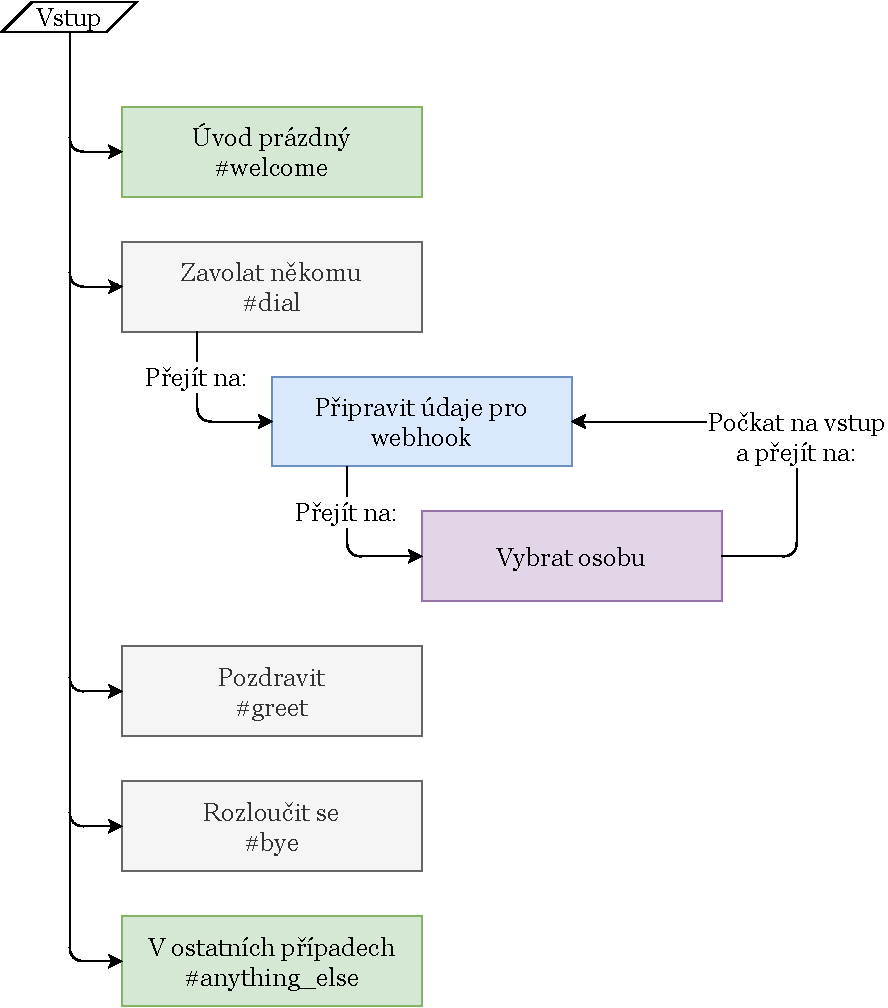
\includegraphics[width=0.7\textwidth]{../img/wa-tree.pdf}
    \caption{Strom dialogu ve WA. Zelené vrcholy detekují vestavěné úmysly,
        šedivé námi definované úmysly, modrý jen vnitřně připravuje data a fialový
        kontaktuje webhook.}
    \label{img-wa-tree}
\end{figure}

\section{Porovnávací komponenta}\label{matching}

Tuto komponentu jsme implementovali pro obecné použití v dialogových systémech
v rámci knihovny \texttt{mConversation} firmy MAMA AI. Za účelem využití v našem
systému jsme komponentě přidali konečné rozhodování, které popisujeme v podsekci~\ref{integration}.
První však v tomto úvodu popíšeme obecné cíle a v podsekcích~\ref{preprocess}~a~\ref{subsection-matching}
vlastní běh komponenty, tedy jak v ní předpřipravujeme data a jak probíhá porovnávání.

Vstupem komponenty jsou entity rozpoznané pomocí WA, původní textový vstup do něj
a určitý (obvykle vázaný na uživatele) seznam entit. Cílem je vybrat entitu ze seznamu,
která nejvíce odpovídá vstupu do WA. V úvahu přitom nejsou brány jen entity, které
WA rozpoznal, ale i originální vstup. Pokud tak například uživatel zmíní běžné jméno a
neběžné příjmení, a WA rozpozná jako entitu jen jméno, komponenta dokáže najít a využít
i příjmení, takže pravděpodobně vrátí pouze jeden kontakt.

Součástí je i příprava pro určité rozšíření využívající strojového učení -- každý
uživatel by měl v budoucnu mít uložený svůj model, který se naučí jeho preference a bude se
průběžně zlepšovat využitím zpětné vazby.

\subsection{Předzpracování}\label{preprocess}

K seznamu kontaktů si vytvoříme slovník,
který jako klíče bude mít všechny části kontaktů a jako hodnoty indexy do původního
seznamu. Tedy například pokud máme v seznamu na prvním místě kontakt \uv{Jan Novák},
ve slovníku budou \uv{Jan} i \uv{Novák} odkazovat na index 1.

Podobně předzpracujeme i rozpoznané entity, pro rychlý přístup k informacím o nich
využijeme opět slovník. Navíc pokud WA rozpoznal dvě entity v navazujících úsecích vstupu,
spojíme je dohromady, pravděpodobně se totiž jedná právě třeba o jméno a příjmení.
Pokud WA v nějakém segmentu rozpoznal více entit a má dojít k tomuto spojování, spojíme
je ve všech různých kombinacích -- například v řetězci \uv{Janě Nové} by mohl
rozpoznat s prvního slova \uv{Jana} i \uv{Jan}, z druhého slova pak \uv{Nový} i
\uv{Nová}, tak bychom vytvořili všechny kombinace \uv{Jana Nová}, \uv{Jana Nový},
\uv{Jan Nový} a \uv{Jan Nová}. Nějaká z nich bude pravděpodobně správná, ale
předem nedokážeme říct, která. Vytvoříme tedy všechny a v dalších krocích
je vyzkoušíme.

\subsection{Vlastní porovnávání}\label{subsection-matching}

Kdykoliv budeme porovnávat nějaké řetězce, využijeme tzv. \textit{fuzzy matching}.
To znamená, že řetězce nebudeme porovnávat přímo, ale pomocí Levenshteinovy vzdálenosti
zmíněné v podsekci~\ref{nlu}. Tím umožníme přiřazení ke kontaktu i při nepřesné shodě,
ať už není shoda úplná kvůli jinému tvaru slova (skloňování), chybě v rozpoznání
hlasu, nebo chybě rozpoznání entity ve WA. Jako odpovídající pak označíme kontakty,
jejichž vzdálenost je menší nebo rovna nějakému limitu. Jako limit maximální vzdálenosti
jsme zvolili 3. Je dost vysoký na to, aby ještě přijal například slovo s příponou
\uv{-ovi}, na druhou stranu vyšší limity způsobují přiřazení i řetězců neodpovídajících,
zvláště u krátkých slov.\footnote{I s tímto limitem můžeme ke slovu délky 3 přiřadit libovolné jiné
    slovo délky 3, protože nám stačí vyměnit 3 znaky. Zlepšení navrhujeme v sekci~\ref{better-match}.}
Pokud celé entitě nalezené v transkripci uživatelova vstupu nic neodpovídá,
zkusíme ji rozdělit na slova a porovnat s telefonním seznamem jednotlivá slova.

Každému přiřazenému kontaktu pak ještě určíme \textit{jistotu} (\textit{confidence}),
s jakou jsme ho přiřadili. Tu jsme se rozhodli počítat jako
\[ \text{jistota} = 0,5 + \frac{0,5 \cdot (\text{limit\_úprav} - \text{vzdálenost})}{\text{limit\_úprav}} ,\]
protože pak řetězce odpovídající přesně dostávají plnou jistotu, zatímco řetězce na
hraně limitu jistotu poloviční. Určitou jistotu navíc entitě přiřadil již WA,
neboť také provádí podobné porovnání. Tyto dvě jistoty navzájem vynásobíme.

Poté ještě vezmeme v úvahu originální vstup, kdyby WA něco nerozpoznal. U každého
úseku vstupu, který byl přiřazen nějakému kontaktu, se díváme na předchozí a následující
slovo, zda neodpovídá stejnému kontaktu. Porovnání uděláme stejně jako v první fázi.
Pokud najdeme slovo, kde tomu tak je, rozšíříme úsek přiřazený k tomuto kontaktu.

Ukážeme
to na příkladu vstupu \uv{chci zavolat Janu Pacušiakovi}, kde WA rozpoznal entitu \uv{Jan}
ke slovu vstupu \uv{Janu} a nic víc, protože příjmení je unikátní a nezná ho.
Naše komponenta pak k této entitě v předchozím kroku přiřadila
kontakty \uv{Jan Novák} a \uv{Jan Pacušiak}, o obou ví zatím jen že odpovídají slovu \uv{Janu}.
V tomto kroku se komponenta dívá na okolní slova.
Zkontroluje slovo \uv{zavolat} a zjistí, že žádný z přiřazených kontaktů mu neodpovídá. Pak
vyzkouší následující slovo \uv{Pacušiakovi} a zjistí, že kontakt \uv{Jan Pacušiak} mu odpovídá,
proto u něj poznačí, že odpovídá celému řetězci \uv{Janu Pacušiakovi}.

Dále z rozpoznání vyřadíme kontakty, které odpovídají jen podúseku jiného
přiřazeného kontaktu. Budeme-li pokračovat s naším příkladem, komponenta vyřadí kontakt \uv{Jan Novák},
protože odpovídá jen slovu \uv{Janu}, zatímco \uv{Jan Pacušiak} odpovídá nadmnožině \uv{Janu Pacušiakovi}.
Vyřadíme také
všechny přiřazené kontakty, jimž jsme udělili jistotu menší než 0,5.

\subsection{Integrace komponenty do systému}\label{integration}

Pro použití v tomto systému potřebujeme, aby komponenta provedla
celé rozhodnutí a pokud si je dostatečně jista, vrátila jen jediný kontakt,
o kterém pak WA předá informaci, že mu má aplikace zavolat. Proto
se podívá na jistoty všech přiřazených kontaktů. Pokud u jednoho
vyjde jistota ostře lepší, vrátí pouze ten. Jako hranici
\uv{ostře lepší} jsme zvolili limit alespoň o 0,1 vyšší než u
ostatních. Pokud žádný ostře lepší nevyjde, vrátíme všechny
nalezené. Pokud jsme nic odpovídajícího nenašli, vrátíme prázdné pole.